\documentclass[12pt]{article}
\usepackage{graphicx}
\usepackage{setspace}
\usepackage{fancyhdr}
\usepackage{amssymb}
\usepackage{xcolor}
\usepackage{amsmath}
\usepackage{svg}
\usepackage[colorlinks=true, urlcolor=blue]{hyperref}
\usepackage{graphicx}
\usepackage{makecell}
\usepackage{fontawesome5}
\usepackage[a4paper, margin=1in]{geometry}
\pagestyle{fancy}
\lhead{Strain analysis for the plateau of Iran}
\rhead{Aliakbar Zarkoob}

\begin{document}
	
	\begin{titlepage}
		\begin{center}
			
			\includegraphics[height=4cm]{University_of_Tehran_Transparent_BW_logo.png} \hfill
			\includegraphics[height=4cm]{Fanni_Alt_BW_Logo.png}
			
			\vspace{1cm}
			
			\Large \textbf{School of Surveying and Geospatial Engineering}\\
			\large {Department of Geodesy and Hydrography}
			
			\vspace{3cm}
			
			\huge \textbf{Strain analysis for the plateau of Iran} \\
			\large \href{https://github.com/XIVAliakbarZarkoob/Strain-Analysis}{\faGithub}
			
			\vspace{2cm}
			
			\Large \textbf{Author:}\\
			\Large Aliakbar Zarkoob
			
			\vspace{2cm}
			
			\Large \textbf{Professor:}\\
			Dr. Sami Samiei Esfahany
			
			\vfill
			
			\large {Autumn 2024}
			
		\end{center}
	\end{titlepage}
	
	
	\section{Introduction}
	
	The Iranian Plateau  is at the collision zone of the Arabian and Eurasian tectonic plates. It's an active region characterized by severe crustal deformation due to ongoing continental collision. It produces widespread seismicity, orogenesis, and lateral shortening, making it a significant place for the investigation of plate tectonics and earthquake hazard. Strain analysis, quantifying the relative deformation of the Earth's crust, is a fundamental geodynamic tool to interpret such processes. From geodetic observations such as Global Positioning System (GPS) displacements or velocities, the strain tensor provides insight into the spatial distribution of extension, compression, shear, and rotation, enabling active deformation patterns to be mapped.
	
	Advancements in geodetic technologies have increased the density and precision of displacement and velocity data, transforming the ability to model crustal strain. As highlighted in foundational works on geodynamics. Strain tensor emerges directly from the displacement gradient, encapsulating both finite and infinitesimal deformations.
	
	This report focuses on the computation and visualization of strain tensors across the Iranian Plateau using finite difference methods applied to GPS velocity observations. The study domain covers a latitudinal range of $24^\circ$ to $43^\circ$ $N$ and a longitudinal extent of $40^\circ$ to $64^\circ$ $E$, creating a regular grid with a $0.25^\circ$ spacing. The methodology is based on strain tensor formulations, including the Eulerian finite strain tensor and 2D approximations for normal strains ($\epsilon_{xx}, \epsilon_{yy}$), shear strain ($\epsilon_{sy}$), and rotation ($\omega$).

	\section{Methodology}
	
	As mentioned before, the aim of this project is to calculate the strain tensor inside a regular grid with latitudinal range of $24^\circ$ to $43^\circ$ $N$ and a longitudinal range of $40^\circ$ to $64^\circ$ $E$, with a $0.25^\circ$ step size. The data used for this project are velocities from 399 GPS stations. These observations are shown in figure \ref{fig:GPSVel}, also the mentioned grid is shown in figure \ref{fig:Grid}.
	
	\begin{figure}[h!]
		\centering
		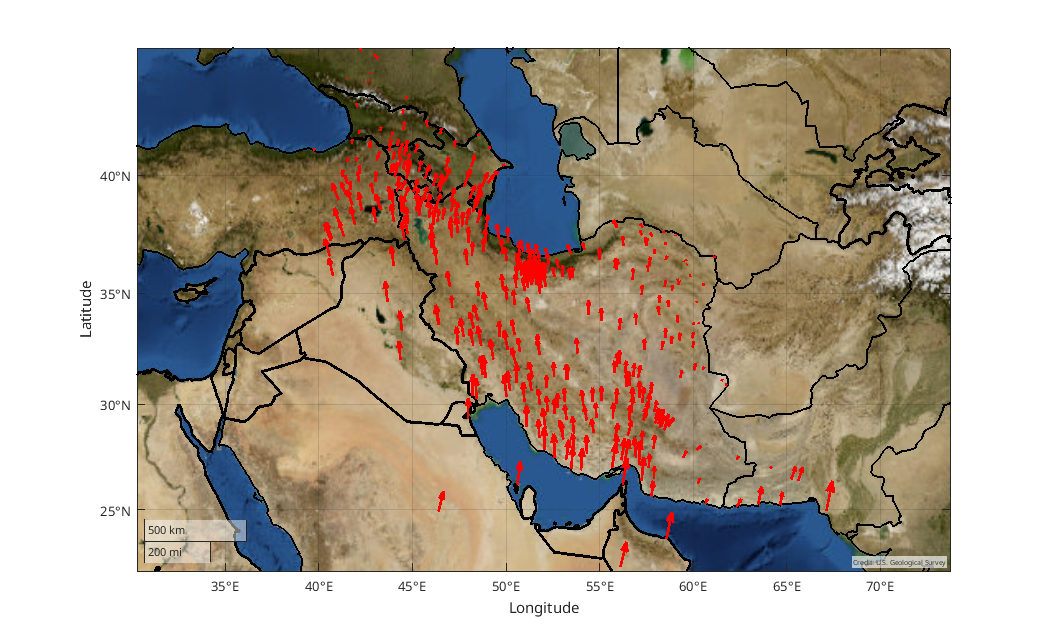
\includegraphics[height=8cm]{./Plots/VelocityMap.pdf}
		\caption{GPS velocity field relative to the Eurasian fixed frame.}
		\label{fig:GPSVel}
	\end{figure}
	
	\begin{figure}[h!]
		\centering
		\includegraphics[height=8cm]{./Plots/Grid.pdf}
		\caption{Study grid for calculation of strain tensors.}
		\label{fig:Grid}
	\end{figure}
	
	The strain tensor is calculated for each point of this grid based on finite difference method shown in the equation \ref{eq:method}. also, the matrix form of these equations are shown in equation \ref{eq:methodmat}.
	
	\begin{equation}
		\begin{cases}
			\dot{u}_{i,x} = \Delta x_i \dot{\epsilon}_{xx} + \Delta y_i \dot{\epsilon}_{xy} + \Delta y_i \dot{\omega} + \dot{d_x} \\ 
			\dot{u}_{i,y} = \Delta x_i \dot{\epsilon}_{xy} + \Delta y_i \dot{\epsilon}_{yy} - \Delta x_i \dot{\omega} + \dot{d_y}
		\end{cases}
		, i=1,2,\dots,m
		\label{eq:method}
	\end{equation}
	
	\begin{equation}
		\underbrace{
			\begin{bmatrix}
				\dot{u}_{1,x} \\[2pt]
				\dot{u}_{1,y} \\[2pt]
				\vdots \\[2pt]
				\dot{u}_{m,x} \\[2pt]
				\dot{u}_{m,y}
		\end{bmatrix}}_{y}
		=
		\underbrace{
			\begin{bmatrix}
				\Delta x_{1} & 0 & \Delta y_{1} & \Delta y_{1} & 1 & 0 \\
				0 & \Delta y_{1} & \Delta x_{1} & -\Delta x_{1} & 0 & 1 \\
				\vdots & \vdots & \vdots & \vdots & \vdots & \vdots \\
				\Delta x_{m} & 0 & \Delta y_{m} & \Delta y_{m} & 1 & 0 \\
				0 & \Delta y_{m} & \Delta x_{m} & -\Delta x_{m} & 0 & 1
		\end{bmatrix}}_{A}
		\underbrace{
			\begin{bmatrix}
				\dot{\varepsilon}_{xx} \\[2pt]
				\dot{\varepsilon}_{yy} \\[2pt]
				\dot{\varepsilon}_{xy} \\[2pt]
				\dot{\omega} \\[2pt]
				\dot{d}_{x} \\[2pt]
				\dot{d}_{y}
		\end{bmatrix}}_{x}
	\label{eq:methodmat}
	\end{equation}
	
	Thus, for each point of the grid, there are $2*399$ observations and $6$ unknowns. In the two equations above, $\dot{u}_{i,x}$ and $\dot{u}_{i,y}$ are the velocity components for the $i$th station. $\Delta x_i$ and $\Delta y_i$ are the difference between the coordinates of a grid point from $i$th station. $\dot{\epsilon}_{xx}$ and $\dot{\epsilon}_{yy}$ are the normal stain rates and $\dot{\epsilon}_{xy}$ is the shear strain rate. also, $\dot{\omega}$, $\dot{d}_{x}$, and $\dot{d}_{y}$ are rotation and displacement components.
	
	An important point is that GPS stations located very far from the grid point under study should not be used in the calculations. In this project, the threshold is defined as the average distance of the GPS stations from the point under study plus 2.5 times their standard deviation.
	
	Now the unknowns ($x$) can be estimated by creating the observation vector ($y$) and design matrix ($A$) with least squares method shown in equation \ref{eq:ls}.
	
	\begin{equation}
		\hat{x} = (A^TWA)^{-1}A^TWy
		\label{eq:ls}
	\end{equation}
	
	In this equation, $W$ is the weight matrix and the way of determining this matrix directly affects the results of estimation. Three parts are included in this matrix as shown in equation \ref{eq:weight}.
	
	\begin{equation}
		W = C^{-1}LZ
		\label{eq:weight}
	\end{equation}
	
	In this equation, $C$ is the covariance matrix of observations, $L$ is weighting based on distance, and $Z$ is weighting based on clustering. Distance weighting is based on a Gaussian function shown in equation \ref{eq:gaussian}.
	
	\begin{equation}
		L_i = e^{-\frac{R_i^2}{D^2}}
		\label{eq:gaussian}
	\end{equation}
	
	Based on this function, the further the stations are the smaller weight is attributed. $R_i$ in this equation is the distance between the grid point and $i$th station. Also, the parameter $D$ is defined as shown in figure \ref{fig:D}.
	
	\begin{figure}[h!]
		\centering
		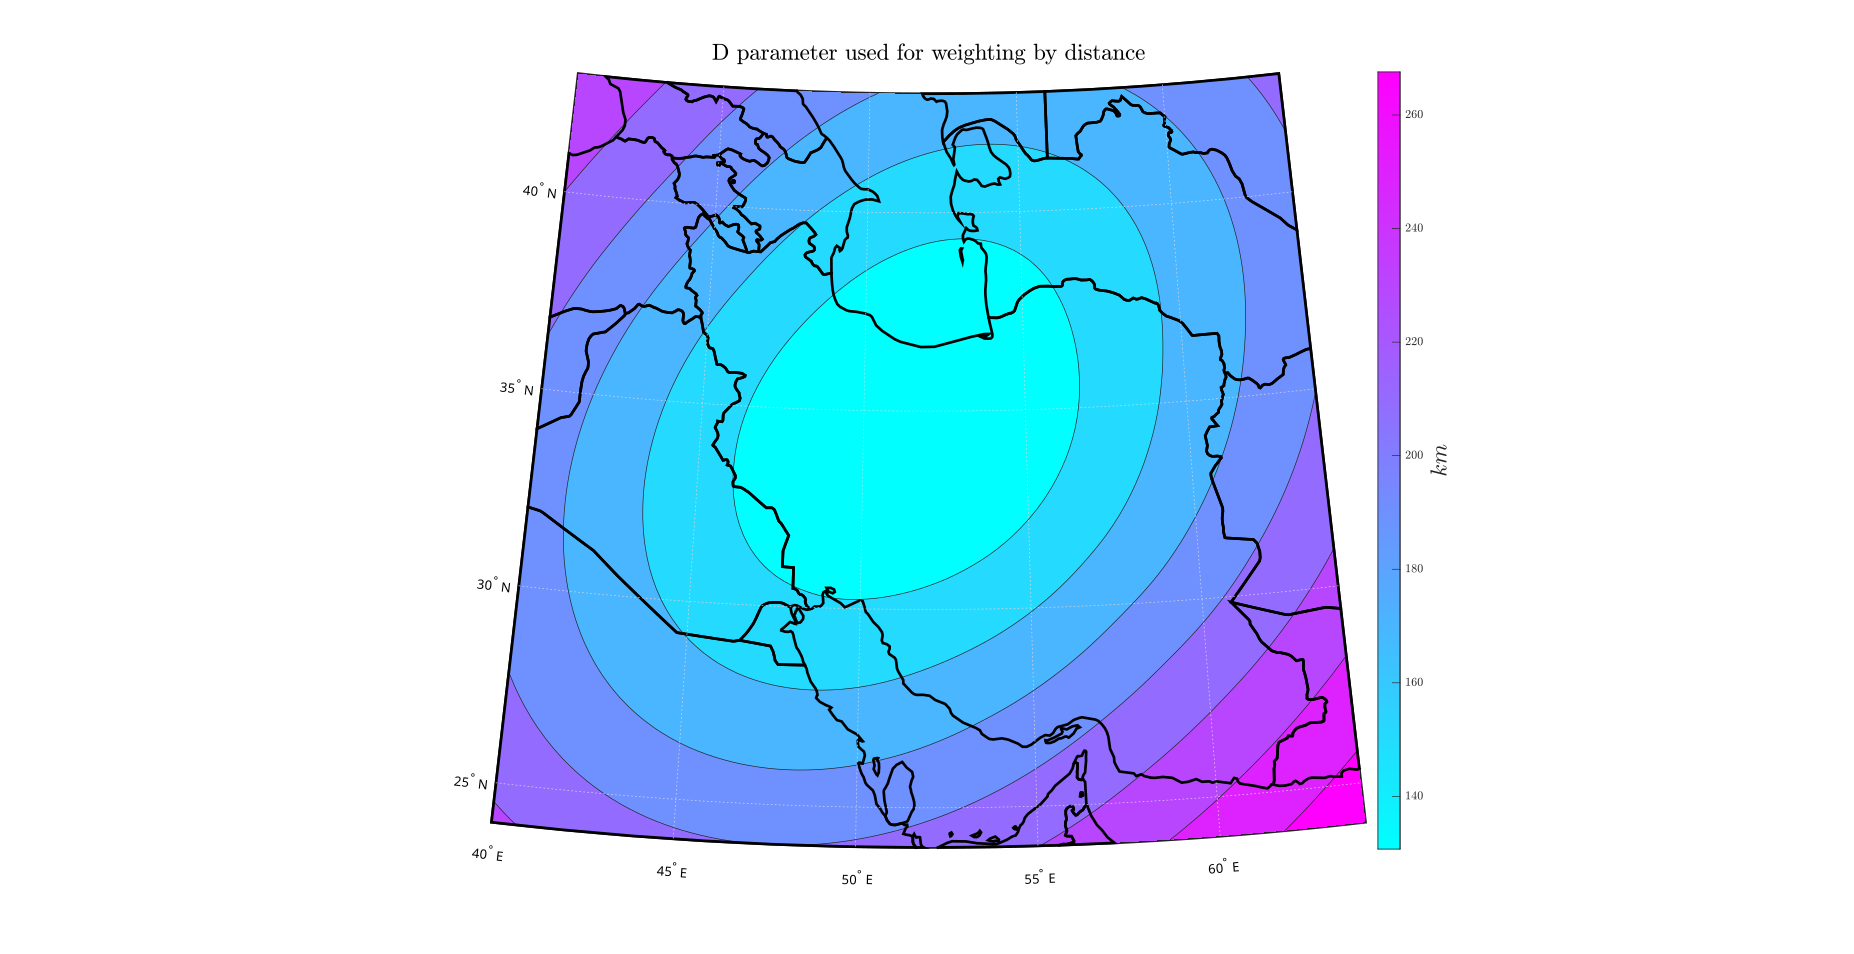
\includegraphics[height=7cm]{./Plots/DWeight.pdf}
		\caption{D parameter for weighting based on distance.}
		\label{fig:D}
	\end{figure}
	
	Clustering is important in weighting due to the fact that areas with more density of stations will bias the result estimations. This weighting is established based on voronoi diagrams. An example of these diagrams are shown in figure \ref{fig:voronoi}. The weights are calculated base on the equation \ref{eq:voronoi}.
	
	\begin{figure}[h!]
		\centering
		\includegraphics[height=5cm]{./Plots/Voronoi.pdf}
		\caption{Voronoi Diagrams for a part of observations.}
		\label{fig:voronoi}
	\end{figure}
	
	\begin{equation}
		Z_i = \frac{nS_i}{\Sigma{S_i}}
		\label{eq:voronoi}
	\end{equation}
	
	In this equation, $n$ is the total number of voronoi diagrams (399) and $S_i$ is the area of the $i$th diagram. Now that the weight matrix is defined, estimated values of the unknowns can be calculated based on the equation \ref{eq:ls}.
	
	After estimating the unknowns, the next step is to calculate the first and second invariants as well as the principal strains for plotting the strain ellipse. The first and second invariants can be computed using equation \ref{eq:invariants}.
	
	\begin{equation}
		\begin{cases}
			I_1 &= \epsilon_{xx} + \epsilon_{yy}\\
			I_2 &= \epsilon_{xx} \epsilon_{yy} - \epsilon_{xy}^2
		\end{cases}
		\label{eq:invariants}
	\end{equation}
	
	The principal strains, which are the eigenvalues of the strain matrix, can be calculated for each grid point using MATLAB’s "eig" command applied to the strain matrix. The angle θ, which is needed to draw the strain ellipses, is calculated using equation \ref{eq:angle}.
	
	\begin{equation}
		\theta = \frac{1}{2} \arctan{\left(\frac{2\epsilon_{xy}}{\epsilon_{xx} - \epsilon_{yy}}\right)}
		\label{eq:angle}
	\end{equation}
	
	\section{Results}
	
	The main products of this project are the different maps. Normal strain and Shear Strain maps are shown in figures \ref{fig:NormalStrain} and \ref{fig:ShearStrain}. Stain Invariants and Principal Strain maps are shown in figures \ref{fig:Invariants} and \ref{fig:Principal}. Lastly, the map of strain ellipses is shown in figure \ref{fig:Ellipse}.
	
	\begin{figure}[h!]
		\centering
		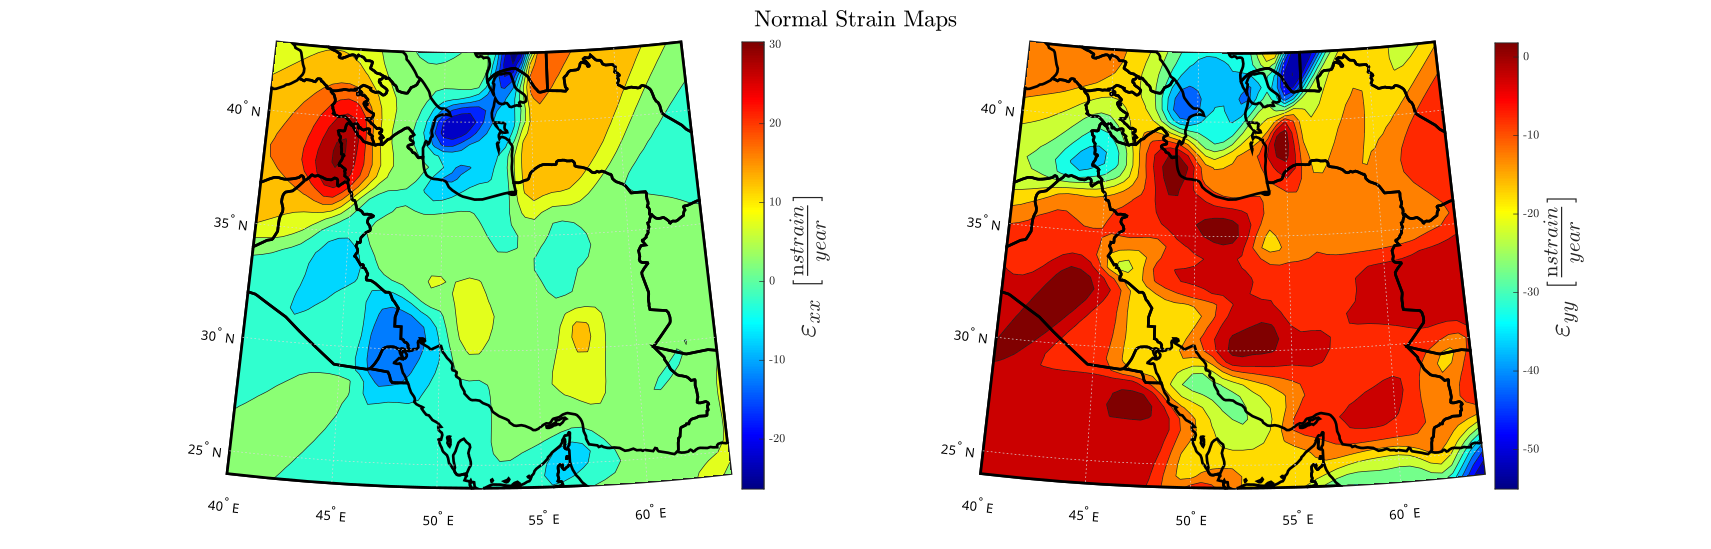
\includegraphics[height=5.5cm]{./Plots/NormalStrainMaps.pdf}
		\caption{Normal strain maps.}
		\label{fig:NormalStrain}
	\end{figure}
	
	\begin{figure}[h!]
		\centering
		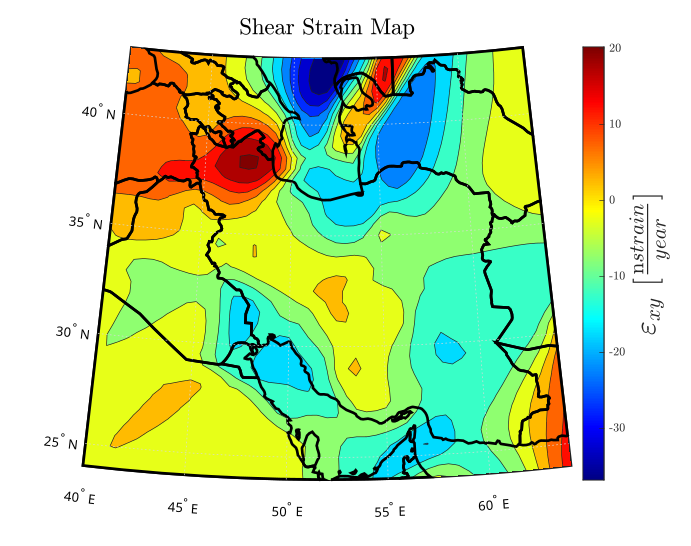
\includegraphics[height=5.5cm]{./Plots/ShearStrainMap.pdf}
		\caption{Shear strain map.}
		\label{fig:ShearStrain}
	\end{figure}
	
	\begin{figure}[h!]
		\centering
		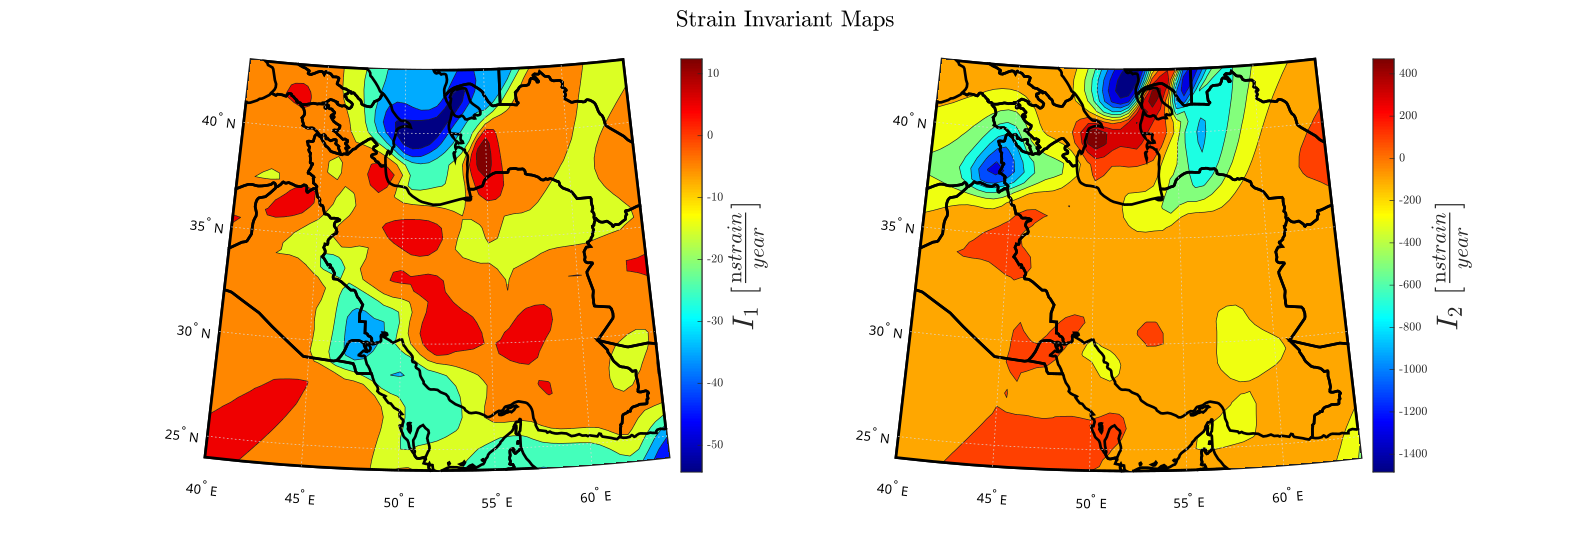
\includegraphics[height=5.5cm]{./Plots/StrainInvariants.pdf}
		\caption{Strain invariants map.}
		\label{fig:Invariants}
	\end{figure}
	

	\begin{figure}[h!]
		\centering
		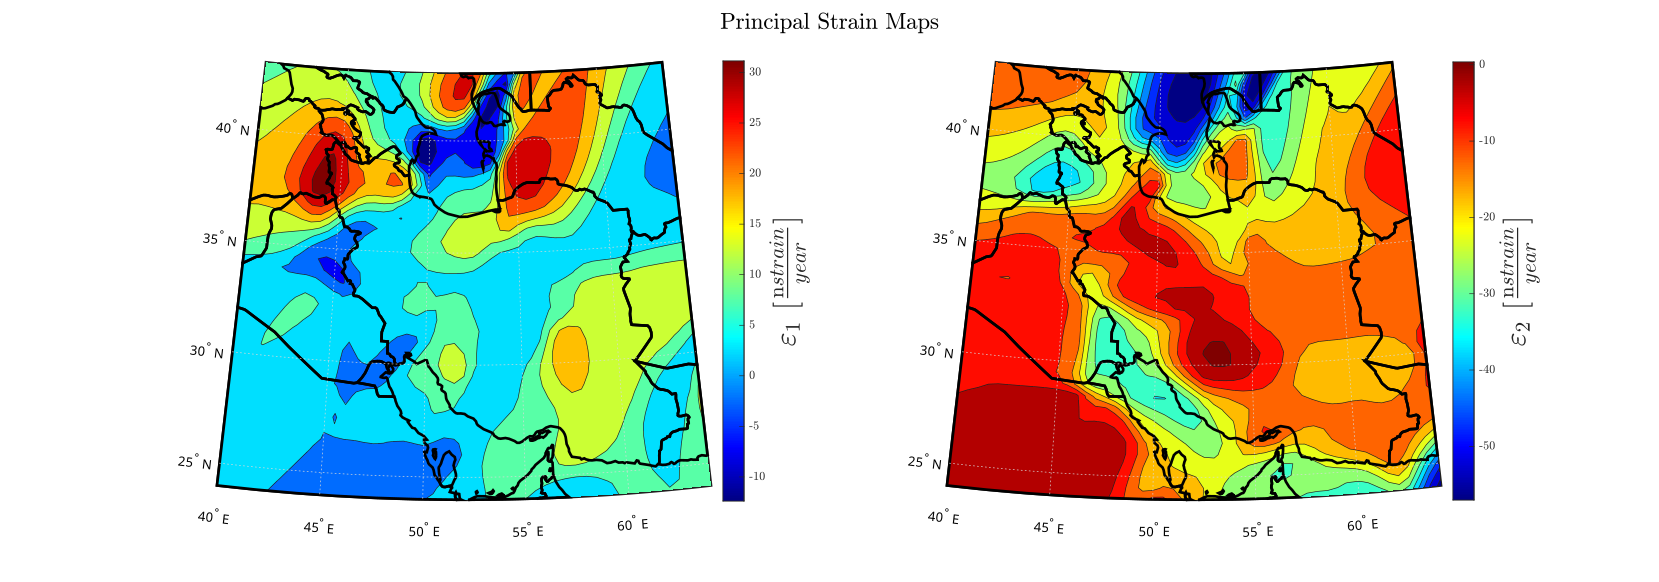
\includegraphics[height=5.5cm]{./Plots/PrincipalStrainMaps.pdf}
		\caption{Principal strain maps.}
		\label{fig:Principal}
	\end{figure}
	\clearpage
	
	\begin{figure}[h!]
		\centering
		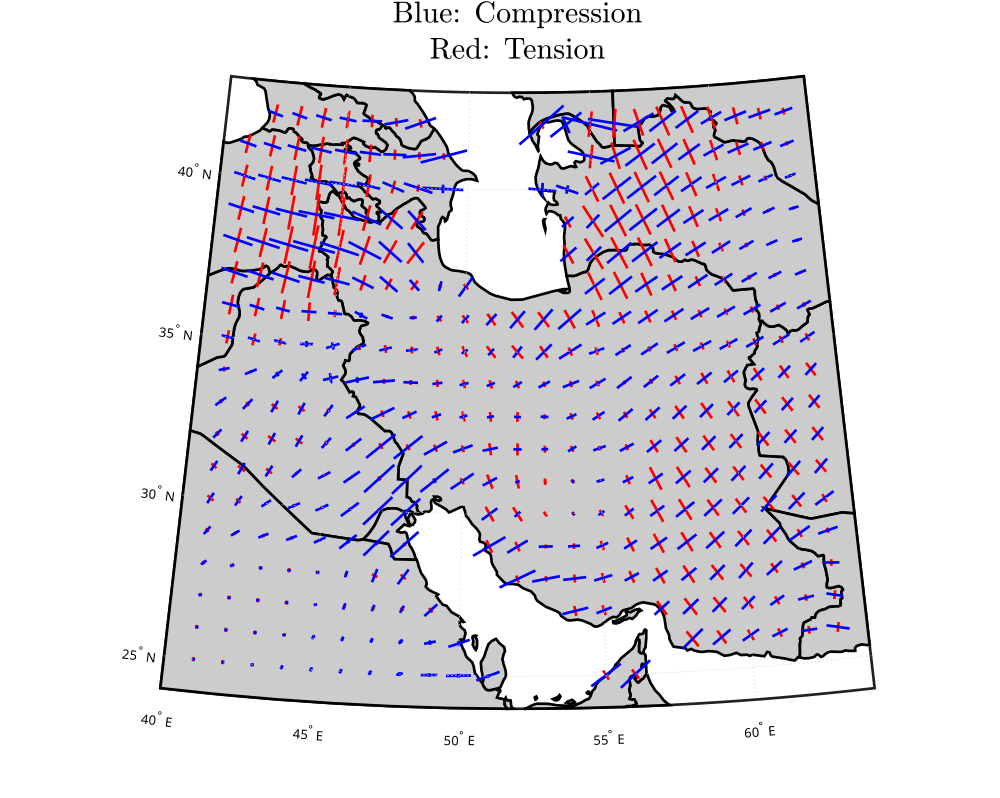
\includegraphics[height=10cm]{./Plots/StrainEllipse.pdf}
		\caption{Strain Ellipses map.}
		\label{fig:Ellipse}
	\end{figure}
	\clearpage
	
\end{document}


